\documentclass[a4paper,11pt,notitlepage]{report}

\usepackage{graphicx}
\usepackage[utf8]{inputenc}
\usepackage[T1]{fontenc}
\usepackage[ngerman]{babel}
\usepackage{bibgerm}
\usepackage{amsmath,amssymb,amsthm}
\usepackage{color}
\usepackage{enumerate}
\usepackage{tabularx}
\usepackage{subfig}
\usepackage{fancyhdr}
\usepackage{upgreek}
\usepackage[pdftex,pdfpagelabels,colorlinks,backref,pagebackref]{hyperref}
\usepackage{tikz} % SELBST HINZUGEFÜGT
\usepackage{lmodern}
\usepackage{subfig}
% == Set the heading style ===================================================
\setlength{\headheight}{14pt}
\pagestyle{fancyplain}
\renewcommand{\chaptermark}[1]{\markboth{#1}{}}
\renewcommand{\sectionmark}[1]{\markright{\thesection\ #1}}
\lhead[\fancyplain{}{\thepage}]{\fancyplain{}{\rightmark}}
\rhead[\fancyplain{}{\leftmark}]{\fancyplain{}{\thepage}}
\cfoot{}
\renewcommand{\headrulewidth}{0.4pt}
% ============================================================================

% == Set correct values for fitting floats ===================================
\tolerance=2000
\emergencystretch=10pt

\setcounter{topnumber}{3}
\setcounter{totalnumber}{5}
\setcounter{bottomnumber}{2}

% To make those darn floats fit where they should
\setcounter{totalnumber}{9}
\setcounter{topnumber}{9}
\setcounter{bottomnumber}{9}
\renewcommand{\textfraction}{0.00}
\renewcommand{\topfraction}{1.0}
\renewcommand{\bottomfraction}{1.0}
% ============================================================================

% == German definitions for theorems etc. ==================================== 
\newtheorem{definition}{Definition}[chapter]
\newtheorem{theorem}{Satz}[chapter]
\newtheorem{lemma}{Lemma}[chapter]
\newtheorem{proposition}{Proposition}[chapter]
\newtheorem{corollary}{Korollar}[chapter]
\newtheorem{observation}{Beobachtung}[chapter]
\newtheorem{fact}{Fakt}[chapter]
\newtheorem{remark}{Bemerkung}[chapter]
\newtheorem{example}{Beispiel}[chapter]
% ============================================================================

% == Abkürzungen für die reellen, natürlichen, ganzen,... Zahlen =============
\newcommand{\R}{{\ensuremath{\mathbb{R}}}}
\newcommand{\N}{{\ensuremath{\mathbb{N}}}}
\newcommand{\Z}{{\ensuremath{\mathbb{Z}}}}
\newcommand{\C}{{\ensuremath{\mathbb{C}}}}
\newcommand{\Q}{{\ensuremath{\mathbb{Q}}}}
\newcommand{\F}{{\ensuremath{\mathbb{F}}}}
\newcommand{\Prim}{{\ensuremath{\mathbb{P}}}}
% ============================================================================

% == Makros für Autorenname und -adresse =====================================
\newcommand{\myaddress}[6]{%
  \parbox{\textwidth}{\textbf{\large #1}\\
    #2\\ #3\\ #4\\ 
    \ifthenelse{\equal{#5}{}}{}{Email: \href{mailto:#5}{\texttt{#5}}\\}
    \ifthenelse{\equal{#6}{}}{}{WWW: \href{#6}{\path|#6|}\\}
  } 
}

\newcommand{\myauthor}[1]{%
  \addtocontents{toc}{\protect\hspace{3.35ex}%
  \textsl{#1}\par}\vspace{-4ex}\quad\hfill\textsl{\Large #1}\vspace{8ex}}

\newcommand{\myname}[1]{\Large #1}

\title{\textbf{{Einführung in die Geometrie und Topologie - Mitschrieb -} \\[5ex] 
    {\Large Übung im Wintersemester 2011/2012\\[5ex]}}}

%%%%%%%%%%%%%%%%%%%%%%%%%%%%%%%%%%%%%%%%%%%%%%%%%%
% Tragen Sie in der folg. Zeile Ihren Namen ein: %
%%%%%%%%%%%%%%%%%%%%%%%%%%%%%%%%%%%%%%%%%%%%%%%%%%
\author{\myname{Sarah Lutteropp}}


\newcommand{\OO}{{\ensuremath{\mathcal{O}}}}

\begin{document}
\shorthandoff{"}
\begin{titlepage}
	\begin{center}	
		\LARGE \textbf{{Einführung in die Geometrie und Topologie - Mitschrieb -} \\[5ex] 
    		{\Large Übung im Wintersemester 2011/2012\\[5ex]}}
	\end{center}
	\begin{center}
		\Large Sarah Lutteropp
	\end{center}
	\begin{center}
		\today
	\end{center}
	\vspace{2cm}
	\begin{center}
		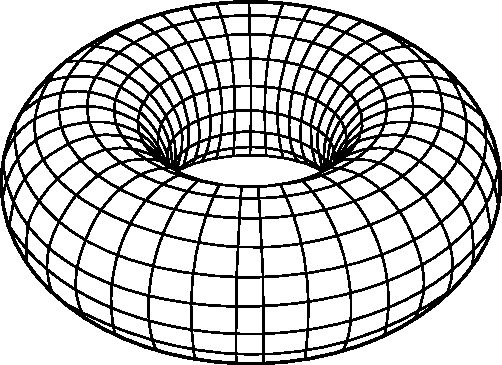
\includegraphics[width=0.8\textwidth]{torus2.pdf}
	\end{center}
\end{titlepage}
%\maketitle
\setcounter{tocdepth}{1}
\tableofcontents

\section*{Vorwort}
Dies ist ein Mitschrieb der Übung “Einführung in die Geometrie und Topologie” vom Wintersemester 2011/2012 am Karlsruher Institut für Technologie, die von Frau Dipl.-Math. Sandra Lenz gehalten wird.

\chapter{24.10.2011}

\begin{section}{Induzierte Topologie}
	\begin{definition}[Induzierte Topologie]
		Sei $X$ eine Menge. Sei $d \colon X \times X \rightarrow \R$ eine Metrik. Diese Metrik $d$ definiert durch folgende Bedingung eine Topologie $\OO$ auf $X$:
		\newline
		$O \subseteq X$ ist genau dann offen (d.h. $O \in \OO_d$), wenn für alle $x \in O$ ein $\epsilon > 0$ existiert mit
		$$
			B_\epsilon (x) := \{y \in X \mid d(x,y) < \epsilon\} \subseteq O.
		$$
		($B_\epsilon$ nennt man offenen $\epsilon$-Ball.)
	\end{definition}
\end{section}

\begin{section}{Offen und abgeschlossen}
	Sei $X$ eine Menge.
	\begin{itemize}
		\item Mengen können sowohl offen als auch abgeschlossen (zugleich) sein.
			\begin{example}
				Betrachte $\emptyset$ und $X$ in der trivialen Topologie $\OO = \{X, \emptyset\}$.
					\newline
					Es gilt: $X \in \OO, \emptyset \in \OO$ nach Definition, d.h. $X$ und $\emptyset$ sind offen.
					\newline
					Außerdem gilt: $X^c = \emptyset \in \OO$, ebenso: $\emptyset^c = X \in \OO$, d.h. die Komplemente von $X$ und $\emptyset$ sind offen und somit $X$ und $\emptyset$ abgeschlossen.
			\end{example}
			
		\item Mengen können weder offen noch abgeschlossen sein.
			\begin{example}
				Betrachte $\R$ mit der von der Standardmetrik induzierten Topologie. Es ist $[0,1[$ nicht offen in dieser Topologie, denn für den Punkt $0$ finden wir kein $\epsilon > 0$, so dass $B_\epsilon(0)$ in $[0,1[$ liegt.
				Die Menge $[0,1[$ ist aber auch nicht abgeschlossen, da ihr Komplement $\R \backslash [0,1[ = ]-\infty,0[ \cup [\underline{1},\infty[$ nicht offen ist.
			\end{example}
		\item Bilder offener Mengen unter stetigen Abbildungen müssen nicht notwendigerweise offen sein.
			\begin{example}
				Betrachte $\R$ mit der von der Standardmetrik induzierten Topologie.
				\newline
				Definiere $f \colon \R \rightarrow \R, x \mapsto x^2$.
				\newline
				Es gilt für die in $\R$ offene Menge $]-1,1[$:
				\newline
				$f(]-1,1[)=[0,1[$ und $[0,1[$ ist nicht offen in $\R$.
			\end{example}
	\end{itemize}
\end{section}

\begin{section}{Basis der von der Standardmetrik auf dem $\R^n$ definierten Topologie}
	$$\mathcal{B} = \{B_{\frac{1}{m}}(x) \mid x \in \Q^n, m \in \N\}$$
	Diese Basis ist abzählbar.
\end{section}

\begin{section}{Teilraumtopologie}
	Es sei $(X, \OO)$ ein topologischer Raum, $A \subseteq X$.
	\newline
	Die Teilraumtopologie (oder Spurtopologie) ist definiert durch
	$$\OO \big |_{A} := \{U \cap A \mid U \in \OO\} $$
	
	\begin{theorem}
		In der Tat definiert $\OO \big |_{A}$ eine Topologie auf $A$.
	\end{theorem}
	
	\begin{proof}
			$\bullet$\underline{z.z.}: Für jede Indexmenge $I$ gilt:
				$\forall i \in I \colon O_i \in \OO \big |_{A} \Rightarrow \bigcup\limits_{i \in I}{O_i} \in \OO \big |_{A}.$
			\newline
			Sei $I$ beliebige Indexmenge. Für alle $i \in I$ mit $O_i \in \OO \big |_{A}$ gilt:
			Es existieren $\mathcal{U}_i \in \OO$ mit $O_i= \mathcal{U}_i \cap A$.
			Es gilt:
			$$\bigcup\limits_{i \in I}{O_i} = \bigcup\limits_{i \in I}{(\mathcal{U}_i \cap A) } = (\bigcup\limits_{i \in I}{\mathcal{U}_i})\cap A \in \OO \big |_{A}$$ (da $\bigcup\limits_{i \in I}{\mathcal{U}_i} \in \OO$).
			\newline
			$\bullet$ \underline{z.z.}: $\forall O_1, O_2 \in \OO \big |_{A} \colon O_1 \cap O_2 \in \OO \big |_{A}.$
			\newline
			Seien $O_1, O_2 \in \OO \big |_{A}$. Dann ex. $\mathcal{U}_1, \mathcal{U}_2 \in \OO$ mit $O_i = \mathcal{U}_i \cap A, i \in \{1,2\}.$ Es gilt:
			$O_1 \cap O_2 = (\mathcal{U}_1 \cap A) \cap (\mathcal{U}_2 \cap A) = (\mathcal{U}_1 \cap \mathcal{U}_2) \cap A \in \OO \big |_{A} \text{, da } \mathcal{U}_1 \cap \mathcal{U}_2 \in \OO.$
			\newline
			$\bullet$ \underline{z.z.}: $A, \emptyset \in \OO \big |_{A}.$
			\newline
			Es gilt: $A = X \cap A \in \OO \big |_{A}\text{, da } X \in \OO$ nach Definition von $\OO$. 
			\newline
			Es gilt: $\emptyset = \emptyset \cap A \in \OO \big |_{A} \text{, da } \emptyset \in \OO$ nach Definition von $\OO$.
	\end{proof}
\end{section}

\begin{section}{Homotopieäquivalenz}
	\begin{definition}
		Seien $X,Y$ topologische Räume. $X$ heißt \underline{homotopieäquivalent zu Y}, falls es stetige Abbildungen $f \colon X \rightarrow Y$ und $g \colon Y \rightarrow X$ gibt, so dass $f \circ g \simeq id_Y$ und $g \circ f \simeq id_X$.
	\end{definition}
	
	\begin{theorem}
		$\R^n \backslash \{0\}$ ist homotopieäquivalent zur Sphäre $S^{n-1}$.
	\end{theorem}
	
	\begin{proof}
		Sei $f \colon S^{n-1} \hookrightarrow \R^n \backslash \{0\}, x \mapsto x$ (Inklusionsabbildung). Dann ist $f$ stetig.
		\newline
		Sei weiter $g \colon \R^n \backslash \{0\} \rightarrow S^{n-1}, x \mapsto \frac{x}{||x||}$. Dann ist auch $g$ stetig und es gilt:
		$g \circ f = id_{S^{n-1}}$, also insbesondere $g \circ f \simeq id_{S^{n-1}}$.
		\newline
		Für $f \circ g$ betrachte folgende Abbildung:
		$$H \colon \R^n \backslash \{0\} \times [0,1] \rightarrow \R^n \backslash \{0\}, (x,t) \mapsto (1-t) \frac{x}{||x||} + t \cdot x$$
		Dann ist $H$ stetig und es gilt für alle $x \in \R \backslash \{0\}$:
		\newline
		$H(x,1) = x = id_{\R^n \backslash \{0\}}(x)$
		\newline
		$H(x,0) = \frac{x}{||x||} = (f \circ g)(x)$
		\newline
		Dann ist $H$ Homotopie von $f \circ g$ nach $id_{\R^n \backslash \{0\}}$ (in Zeichen: $f \circ g \simeq id_{\R^n \backslash \{0\}}$).
	\end{proof}
\end{section}

\chapter{31.10.2011}
\section{Universelle Eigenschaft der Teilraumtopologie}
Es sei $(X, \OO_X)$ ein topologischer Raum und $A \subseteq X$ versehen mit der Teilraumtopologie $\OO_A = \{ O \cap A \mid O \in \OO_X \}$. 
Weiter sei $\iota \colon A \hookrightarrow X$ die Inklusionsabbildung und $(Y, \OO_Y)$ ein weiterer topologischer Raum.

\begin{theorem}{Behauptung}
Eine Abbildung $\phi \colon Y \rightarrow A$ ist genau dann stetig, wenn die Komposition $\iota \circ \phi \colon Y \rightarrow X$ stetig ist.
\end{theorem}

\begin{proof}
`$\Rightarrow$': Es sei $\phi \colon Y \rightarrow A$ stetig. [\underline{z.z.}: $\iota \circ \phi$ ist stetig, d.h. $\forall O \in \OO_X \colon (\iota \circ \phi)^{-1}(O) \in \OO_Y$]
\newline
Sei $O \in \OO_X$. Dann gilt $(\iota \circ \phi)^{-1}(O) = \phi^{-1}\left(\iota^{-1}(O)\right)$ und es ist $\iota^{-1}(O) \in \OO_A$, da $\iota$ stetig ist.
\newline
Es gilt somit $\phi^{-1}\left(\iota^{-1}(O)\right) \in \OO_Y$, da $\phi$ stetig ist (nach Voraussetzung).
\newline
`$\Leftarrow$': Es sei $\phi \colon Y \rightarrow A$ eine Abbildung, so dass $\iota \circ \phi \colon Y \rightarrow X$ stetig ist. [\underline{z.z.}: $\phi$ ist stetig, d.h. $\forall O \in \OO_A \colon \phi^{-1}(O) \in \OO_Y$.]
\newline
Sei also $O \in \OO_A$. Dann existiert $O^\prime \in \OO_X$, so dass $O = O^\prime \cap A$.
Es gilt: $\iota^{-1}(O^\prime) = O^\prime \cap A = O$.
\newline
$\phi^{-1}(O) = \phi^{-1}(O^\prime \cap A) = \phi^{-1}\left(\iota^{-1}(O^\prime)\right) = (\iota \circ \phi)^{-1}(O^\prime) \in \OO_Y$, da $\iota \circ \phi$ stetig (nach Voraussetzung).
\end{proof}

\begin{remark}{(Bemerkung in der Vorlesung)}

Die Teilraumtopologie ist die gröbste Topologie, bezüglich der die Inklusionsabbildung $\iota \colon A \hookrightarrow X$ stetig ist.
\end{remark}

\begin{proof}
\underline{Stetigkeit der Inklusionsabbildung}: [\underline{z.z.}: $\forall O \in \OO_X \colon \iota^{-1}(O) \in \OO_A$]
\newline
Sei $O \in \OO_X$. Dann gilt $\iota^{-1}(O)=O \cap A \in \OO_A$.
\end{proof}


\begin{proof}
\underline{Nichtstetigkeit in gröberen Topologien}: [\underline{z.z.}: $\OO_A \not\subseteq \tilde \OO \Rightarrow \exists O^\prime \in \OO_X \colon \iota^{-1}(O^\prime) \notin \tilde \OO$]
\newline
Sei $\OO_A \not\subseteq \tilde \OO \Rightarrow \exists O \in \OO_A\colon O \notin \tilde\OO$. Dann  $\exists O^\prime \in \OO_X \colon O = O^\prime \cap A$. Damit ist aber $\iota^{-1}(O^\prime)=O^\prime \cap A = O \notin \tilde\OO \Rightarrow \iota\colon (A,\tilde\OO) \rightarrow (X,\OO_X)$ ist nicht stetig.
\end{proof}

\section{Homöomorphismen}
Zeigen Sie, dass für $a,b \in \R$ mit $a < b$ das Intervall $(a,b)$ homöomorph zum Intervall $(0,1)$ ist, sowie dass $(0,1)$ homöomorph ist zu $\R$.
\newline
Definiere $f \colon (a,b) \rightarrow (0,1), x \mapsto \frac{a-x}{a-b}$, und $g \colon (0,1) \rightarrow (a,b), x \mapsto (1-x) \cdot a + x \cdot b$.
\newline
Es gilt für alle $x \in (a,b)$:
\newline
$(g \circ f)(x) = g \left(\frac{a-x}{a-b}\right) = \left(1- \frac{a-x}{a-b}\right)a + \frac{a-x}{a-b}b = \left(\frac{a-b-a+x}{a-b}\right)a+ \frac{a-x}{a-b}b = \frac{x-b}{a-b}a + \frac{a-x}{a-b}b = \frac{ax-ab+ab-bx}{a-b} = x$.
\newline
Es gilt für alle $x \in (0,1)$:
\newline
$(f \circ g)(x)=f\left((1-x) \cdot a + x \cdot b\right)=\frac{a-((1-x)a+bx)}{a-b}=\frac{a-a+ax-bx}{a-b}=x$. Somit ist $f$ bijektiv. 
Da $f$ und $g = f^{-1}$ stetig sind, gilt damit: $f$ ist ein Homöomorphismus, d.h. $(a,b) \equiv (0,1)$.
\newline
Definiere $h \colon (0,1) \rightarrow \R, x \mapsto \tan{\left((x-\frac{1}{2})\pi \right)}$.
\newline
\newline
$f \colon [0,1) \rightarrow S^1, t \mapsto e^{2\pi i t} \left(=(\cos{2 \pi t}, \sin{2 \pi t})\right)$ ist kein Homöomorphismus (da die Umkehrabbildung nicht stetig ist).

\begin{figure}[h]
\centering
\subfloat[$f$ ist stetig $\dots$]{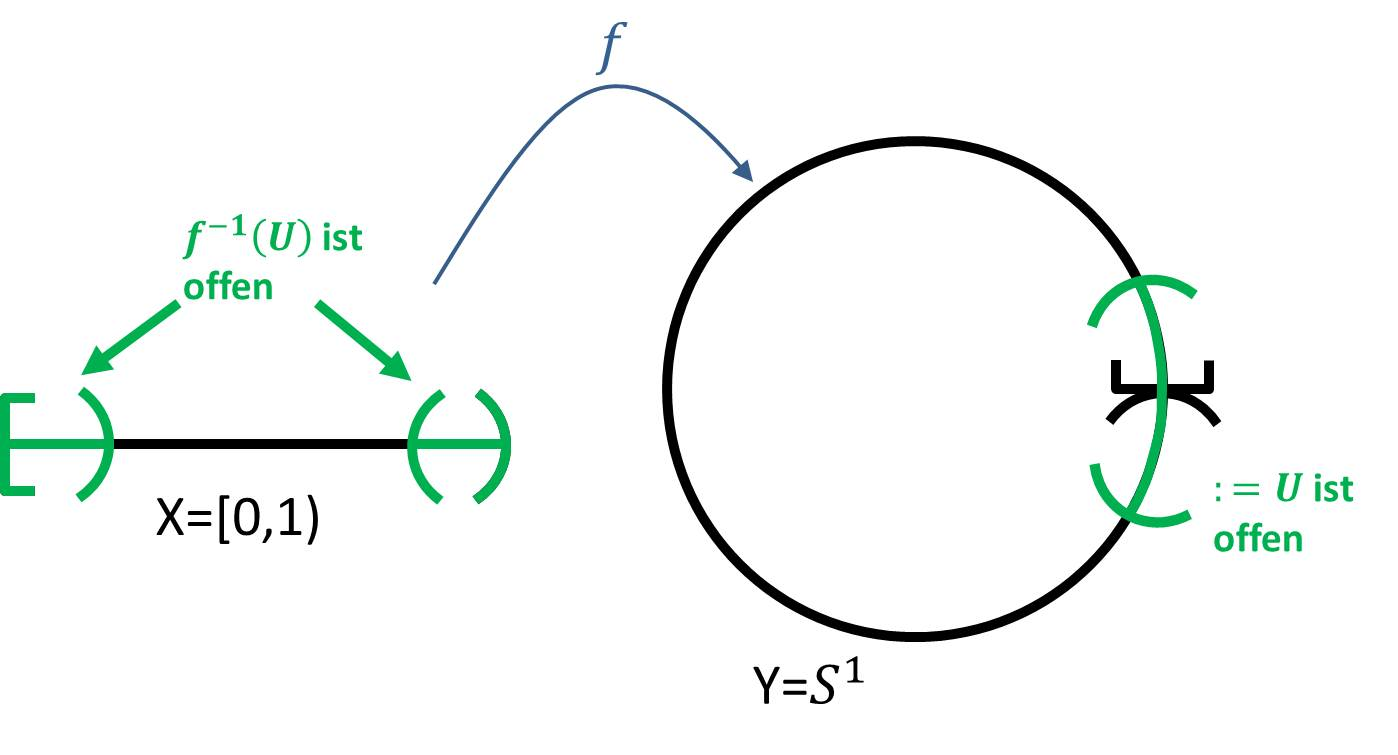
\includegraphics[width=0.75\textwidth]{images/0_1_nach_S1_f_stetig.jpg}}
\subfloat[$\dots f^{-1}$ aber nicht.]{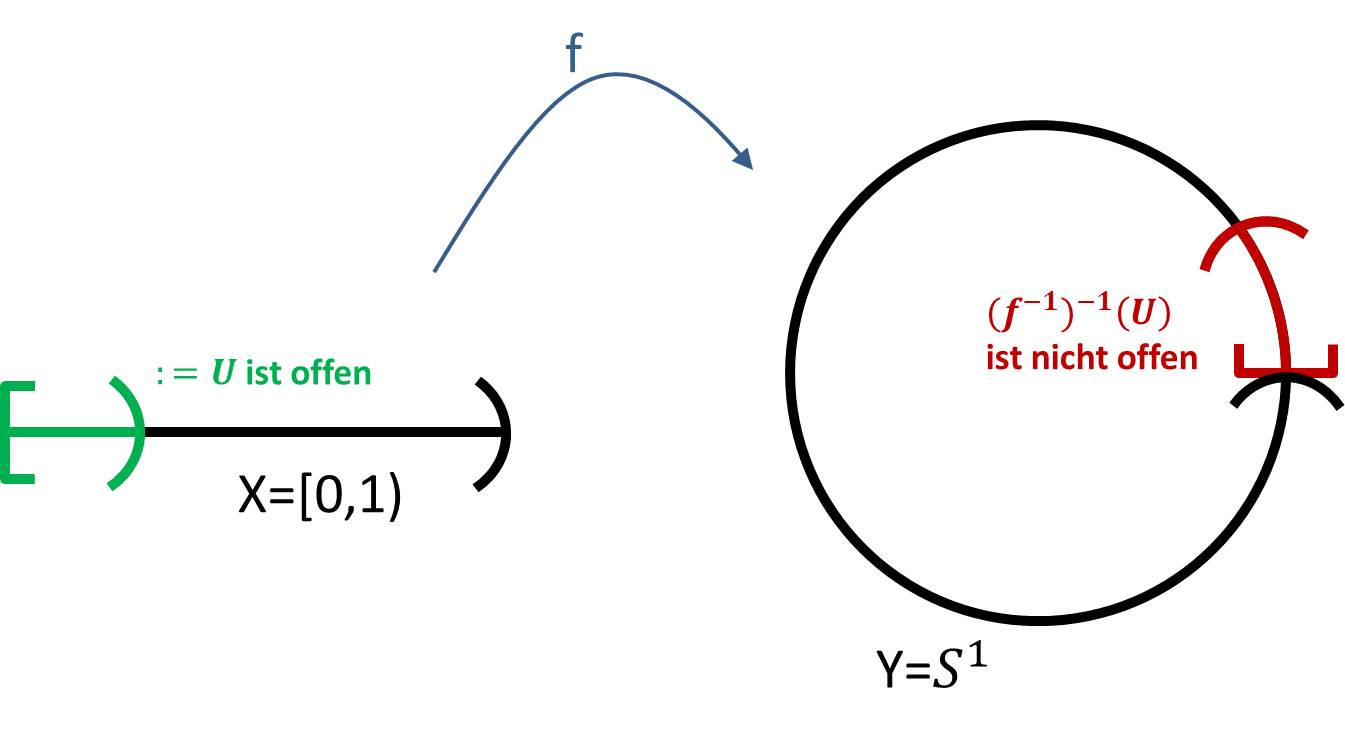
\includegraphics[width=0.75\textwidth]{images/0_1_nach_S1_f-1_nicht_stetig.jpg}}
\end{figure}

\section{Die Peano-Kurve}
(Guiseppe Peano, $\sim 1890$)
\begin{theorem}
	Es gibt eine surjektive, stetige Abbildung $I = [0,1] \rightarrow I \times I$.
\end{theorem}

\begin{figure}[h]
\centering
\subfloat[Iteration 1]{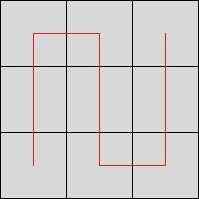
\includegraphics[width=0.4\textwidth]{images/PeanoKurve1.jpg}}\qquad
\subfloat[Iteration 2]{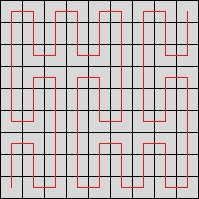
\includegraphics[width=0.4\textwidth]{images/PeanoKurve2.jpg}}
\caption{Prinzip der Peano-Kurve}
\end{figure}

\paragraph{Verallgemeinerung}
\begin{itemize}
\item Es gibt eine surjektive, stetige Abbildung $I \rightarrow I^n = I \times I \times \ldots \times I (n \in \N)$.
\item Es gibt eine surjektive, stetige Abbildung $\R \rightarrow \R^n$.
\end{itemize}

\subsection{Zugang mit Hilfe der Cantor-Menge $\mathcal{C}$}
Definiere $f \colon \mathcal{C} \rightarrow I, f \left(\sum\limits_{i=1}^{\infty}{\frac{a_i}{3}} \right) = \sum\limits_{i=1}^{\infty}{\frac{\frac{a_i}{2}}{2^i}}$ für $a_i \in \{0,2\}$.
\newline
Dann ist $f$ surjektiv und stetig.
\newline
Definiere $g \colon \mathcal{C} \rightarrow \mathcal{C} \times \mathcal{C}, g \left(\sum\limits_{i=1}^{\infty}{\frac{a_i}{3}} \right) = \left(\sum\limits_{i=1}^{\infty}{\frac{a_{2i}}{3^i}}, \frac{a_{2i+1}}{3^i} \right)=:(g_1,g_2)$ für $a_i \in \{0,2\}$.
\newline
Dann ist $g$ surjektiv und stetig.
\newline
Es ist auch $h \colon \mathcal{C} \rightarrow I \times I, x \mapsto \left(f(g_1(x)), f(g_2(x))\right)$ surjektiv und stetig.
\newline
Setze die Abbildung $h$ durch lineare Fortsetzungen stetig auf $I$ fort.
\end{document}
